% !TEX program = xelatex
\documentclass[12pt,a4paper]{article}
\usepackage[T1]{fontenc}
% --- XeLatex/LuaLatex ---
\usepackage[no-math]{fontspec}
\IfFontExistsTF{Fira Sans}{
	\setmainfont{Fira Sans}
}
\usepackage[indonesian]{babel}
\usepackage{booktabs}
%\renewcommand{\familydefault}{\sfdefault}
\usepackage{geometry}
\usepackage{tabularx}
\usepackage{graphicx}
\usepackage{float}
\usepackage{xcolor}
\usepackage{hyperref}
\usepackage{subcaption}
%\usepackage{subfigure}
\hypersetup{
	colorlinks=true,  % Colours links instead of boxes
	urlcolor=blue,    % Colour for external hyperlinks
	linkcolor=blue,   % Colour of internal links (sections, etc.)
	citecolor=red,    % Colour of citations
	hypertexnames=true
}
\geometry{left=2cm, right=2cm, top=2cm}
\title{\textbf{Panduan \textit{Setting} Kamera}}
\author{Observatorium Bosscha}
\hyphenation{me-la-ku-kan peng-amat-an deng-an di-re-ko-men-da-si-kan mem-pe-nga-ruh-i ren-tan peng-ambil-an se-suai-kan me-dan}
\begin{document}
\maketitle
\noindent\rule{\linewidth}{0.4pt}

\setcounter{section}{1}
\subsection*{Catatan Penting}
\begin{itemize}
	\item Setiap kamera memiliki himpunan parameter yang unik. Gunakan dokumen ini sebagai panduan umum dan sesuaikan dengan kamera yang digunakan.
	\item \textcolor{red}{Jangan mengubah parameter pada tab \textbf{Image Controls} karena hal ini akan memengaruhi kalibrasi.} \textit{Setting} default adalah: Gamma=1, Contrast=0, Brightness=0, Timestamp Frames=Off.
	\item Pada tahap ini \textbf{Preprocessing} tidak digunakan.
	\item Target \textit{frame rate} yang ideal adalah lebih dari 30 fps, dengan target minimum 5 fps.
	\item Target SNR (Signal-to-Noise Ratio) yang ideal adalah lebih dari 100, dengan target minimum 10.
	\item Jika target ideal tidak dapat dicapai secara bersamaan, prioritaskan agar SNR tetap memenuhi batas minimum sambil menjaga \textit{frame rate} setinggi mungkin. Jangan gunakan konfigurasi dengan SNR di bawah 10 atau \textit{frame rate} di bawah 5 fps, kecuali tidak ada alternatif lain dan kondisi tersebut dicatat pada log--sheet.
\end{itemize}

\subsection*{1. Capture Format and Area}
\begin{center}
	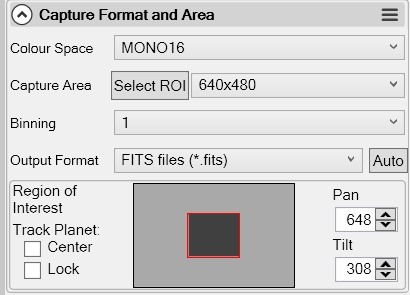
\includegraphics[width=0.4\linewidth]{capture_format_area}
\end{center}

\begin{table}[H]
	\centering
		\begin{tabular}{l l p{12cm}}
		Colour Space & : & \textbf{MONO16}\\
		Capture Area & : & Sesuaikan ukuran ROI agar target \textbf{Frame Rate} tercapai dan medan pandang cukup untuk menangkap bintang target serta bintang-bintang pemandu. Acuan FOV minimum dapat dilihat pada dokumen \textit{Panduan Pengamatan}, Langkah 2, pada \textit{finding chart}.\\
			 && Catatan: semakin besar ROI, semakin rendah \textit{frame rate}. Sesuaikan dengan kebutuhan dan kemampuan perangkat.\\
		Binning & : & \textbf{1 x 1}\\
		Output Format & : & \textbf{FITS files (*.fits)} \\
	\end{tabular}
\end{table}

\subsection*{2. Camera Controls}
\subsubsection*{2.1. Kamera non--GPS (contoh: ZWO ASI290MM)} 
\begin{center}
	\includegraphics[width=0.4\linewidth]{"camera controls"}
\end{center}

\begin{table}[H]
	\centering
	\begin{tabular}{l l p{12cm}}
		Exposure & : & \textbf{5-25 ms (LX Mode \underline{tidak} dicentang)}\\
		&& Catatan: lakukan pengujian dalam rentang nilai ini untuk mencapai target \textit{frame rate} dan SNR.\\
		Gain & : & \textbf{70-75 (rekomendasi awal untuk contoh kamera ini; sesuaikan untuk setiap kamera, sekitar 70-75\% dari total gain)} \\
		Frame Rate Limit & : & \textbf{Maximum}\\
		Turbo USB & : & \textbf{40-80}\\
		&& Catatan: semakin tinggi nilai USB Traffic, semakin cepat transfer data, tetapi sistem juga semakin rentan terhadap \textit{drop frames}. Jika ada kendala koneksi atau \textit{drop frames}, kurangi nilai ini hingga hasilnya stabil.\\
		Overclock & : & \textbf{0}\\
		High Speed Mode & : & \textbf{Off}\\
	\end{tabular}
\end{table}

Selama optimasi, parameter yang boleh disesuaikan hanya ROI, \textit{exposure}, gain, dan USB Traffic. Biarkan parameter lain dalam keadaan \textit{default}.

\subsubsection*{2.2. Kamera GPS (contoh: QHY 174M GPS)}
\begin{center}
	\includegraphics[width=0.4\linewidth]{"camera controls_gps"}
\end{center}

\begin{table}[H]
	\centering
	\begin{tabular}{l l p{10cm}}
		Exposure & : & \textbf{5-25 ms (LX Mode \underline{tidak} dicentang)}\\
		&& Catatan: lakukan pengujian dalam rentang nilai ini untuk mencapai target \textit{frame rate} dan SNR.\\
		Gain & : & \textbf{300 (rekomendasi awal untuk QHY 174M GPS; sesuaikan bila menggunakan kamera lain, dengan acuan sekitar 70-75\% dari total gain)} \\
		Frame Rate Limit & : & \textbf{Maximum}\\
		Amp Noise Reduction & : & \textbf{Auto}\\
		Offset & : & \textbf{100}\\
		USB Traffic & : & \textbf{40-80}\\
		&& Catatan: semakin tinggi nilai USB Traffic, semakin cepat transfer data, tetapi sistem juga semakin rentan terhadap \textit{drop frames}. Jika ada kendala koneksi atau \textit{drop frames}, kurangi nilai ini hingga hasilnya stabil.\\
		Enable Live Broadcast & : & \textbf{Off}\\
		Force Still Mode & : & \textbf{Off}\\
	\end{tabular}
\end{table}

\subsection*{3. Image Controls}
\begin{figure}[H]
	\centering
	\begin{minipage}[t]{0.45\textwidth}
		\includegraphics[width=\linewidth]{"image controls"}
		\caption*{ZWO ASI290MM}
	\end{minipage}\hfil
	\begin{minipage}[t]{0.45\textwidth}
		\includegraphics[width=\linewidth]{"image controls gps"}
		\caption*{QHY 174M GPS}
	\end{minipage}
\end{figure}

Semua \textit{setting} dibiarkan dalam keadaan default seperti pada gambar.
%\begin{table}[H]
%	\centering
%	\begin{tabular}{l l p{8cm}}
%		Timestamp frames & : & \textbf{Off}\\
%	\end{tabular}
%\end{table}

\subsection*{4. GPS Controls (untuk QHY 174M GPS)}
\begin{center}
	\includegraphics[width=0.4\linewidth]{"gps control"}
\end{center}
\begin{table}[H]
	\centering
	\begin{tabular}{l l p{8cm}}
			GPS & : & \textbf{On}\\
			Show Data & : & \textbf{On} (digunakan untuk memeriksa status GPS dan sinkronisasi jam komputer sebelum pengambilan data).\\
		\end{tabular}
\end{table}
Jangan ubah parameter lainnya. Pada bagian ini, parameter yang boleh disesuaikan hanya \textit{exposure}, gain, ROI, dan USB Traffic. Biarkan parameter lain dalam keadaan default.

Jika GPS sudah dalam keadaan \textit{locked} (tekan tombol \textbf{Show Data} jika jendela status GPS belum terlihat), tekan tombol \textbf{Set PC Time to GPS Time} sesaat sebelum pengambilan data dilakukan. Jika ada jeda yang cukup lama sebelum perekaman dimulai atau jam komputer diduga berubah, ulangi sinkronisasi ini tepat sebelum perekaman.
\begin{center}
	\includegraphics[width=0.4\linewidth]{"gps status"}
\end{center}

\subsection*{5. Thermal Controls}
\begin{center}
	\includegraphics[width=0.4\linewidth]{"thermal controls"}
\end{center}
\begin{table}[H]
	\centering
	\begin{tabular}{l l p{8cm}}
		Cooler Power & : & \textbf{Auto}\\
		Target Temperature & : & \textbf{0}\\
	\end{tabular}
\end{table}
Pengaturan ini digunakan untuk menjaga temperatur sensor tetap stabil selama pengambilan data tanpa membebani sistem pendingin secara berlebihan.
\end{document}